\chapter{背叛者(十一)}

\section*{前言}
\begin{verse}
安洁在城楼上观山景,耳听得楼下乱纷纷。

旌旗招展空泛影,却是那叶戈尔发来的兵。
\end{verse}

\lineseparator{}


\begin{figure}[htbp]
  \centering
  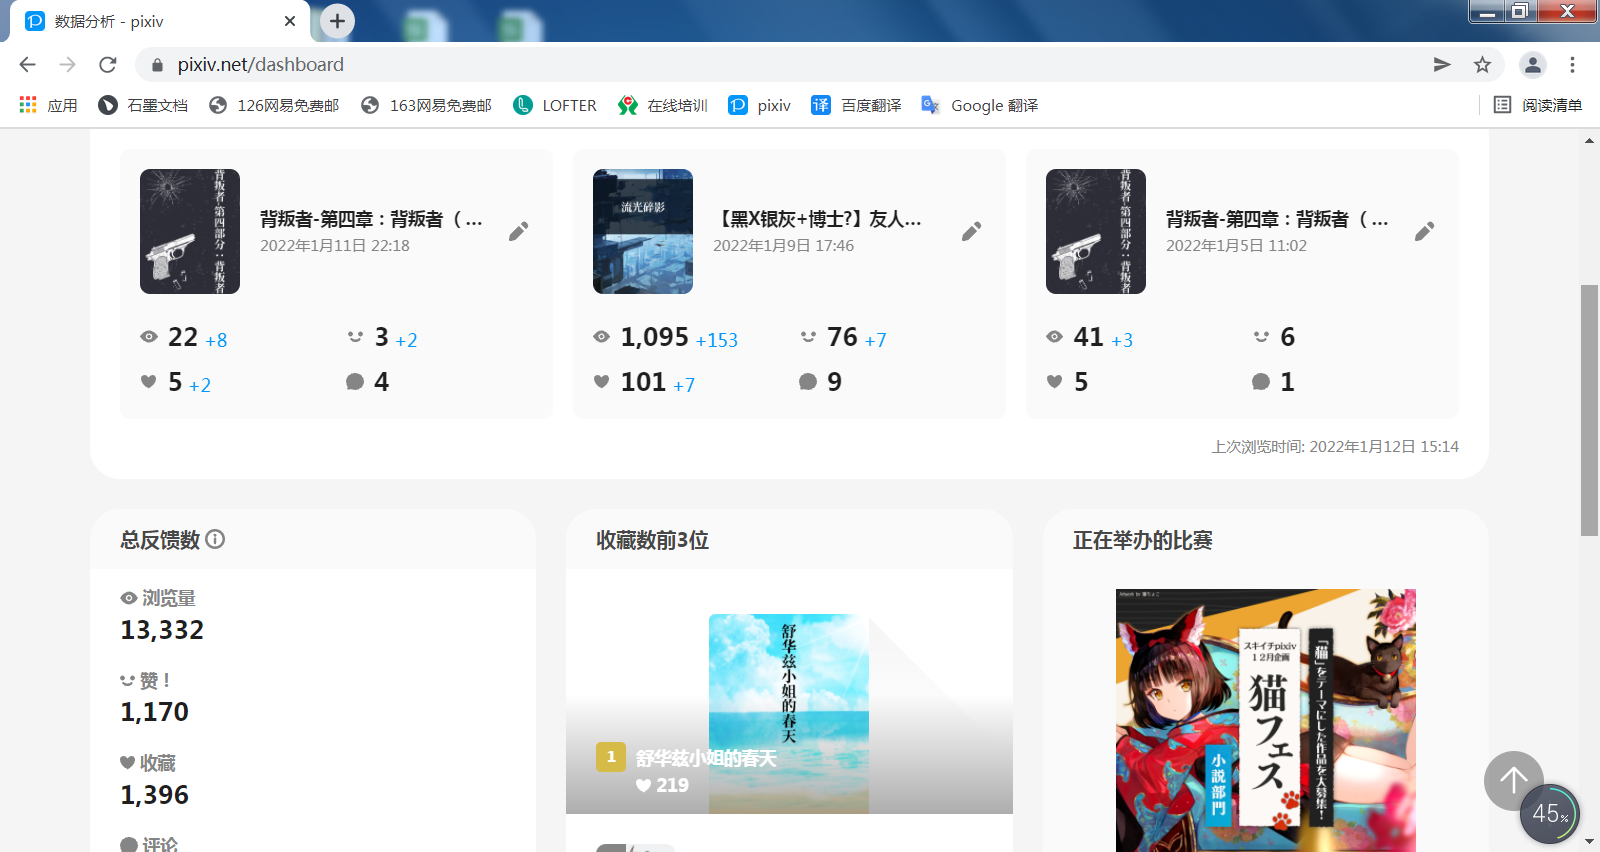
\includegraphics[width=0.7\linewidth]{tei570040063950_ed20dd5e01572ca6287298ecdffa8895.png}
  \caption{作者的Pixiv数据统计图}
  \label{fig:作者的Pixiv数据统计图}
\end{figure}

这点击量和收藏量,高下立判啊……

不想说别的了,赶紧完结这费劲不讨好的玩意去写小黄文吧- -

正文下一页。

\section*{}



战场的另一端——

“安洁,看那个信号弹!”AN94说。几个人抬起头,看到距离不远的地方升起了一颗绿色的信号弹,在夜空中十分醒目。

“是格里芬的信号弹,他们是在指引我们行动的方向!”安洁说。

“可是……那里是红区,安洁。我不认为这是明智的选择。”AK12担忧地说。

“安洁……你恐怕撑不到安全地带。”AN94也说。

“咳……没关系……我愿意再赌一把。”安洁说。

“这可不是靠意志力就能挺过去的事情!”AK12加重了语气说,“仪器显示,这个区域的污染度还在增加,进入红区只会让你的症状更加严重!”

“这座城市里任何地方都有污染,”安洁摇了摇头,“绕开红区吸收的辐射也不会少,除了消耗更多时间外没有其他好处。”

“那就走吧,AK12。感染者增多了,不能拖延下去了。”AN94说道。

“不,我强烈建议绕开红区。”AK12依然反对安洁的决定。

“没时间浪费了!咳咳……”安洁说着剧烈地咳嗽了起来,“AK12,AN94……如果……如果……你们知道……咳……咳咳咳……!咳——!”

“好了,别争了。”一直在旁沉默的陆久开口说道,“安洁的选择是正确的,绕远的话不知道路上会遇到什么,至少格里芬指出的那个方向要相对安全一些。我们必须穿过红区。”

“安洁根本撑不到那时,”AK12说,“她会死在路上的。”

“那就穿上这个。”陆久说着解开防弹衣,然后脱下了自己的防辐射服递给安洁。

“这——”安洁微微睁大了眼睛说道,AK12和AN94也愣住了。

“不要误会。为了让自己活下来,我不会吝惜牺牲你们的。但现在是非常情况。”陆久说,“我没有时间可以浪费,所以必须快点结束这些事情。如果安洁能在辐射中活这么久,那我受点污染,应该也问题不大。所以,就当帮我个忙,快点行动。”

“你这么说,是怕我不肯接受吗?没有必要。”安洁勉强地笑了笑,接过了陆久的防护服,“时间对我来说同样重要。虽说我不忍心为了让自己活下来而牺牲你,但既然是你主动要求,我也就没必要推辞了。”

“呵,请笑纳。”陆久笑了一声说,“不过,这个防护面罩我就自己留着了,我不想让某些人看到我的脸。”

“我能理解。”安洁说着穿上了陆久的防护服,“总之,还是多谢了。这套衣服等穿过红区我就还给你。马上行动吧。”

AK12在最前面开路,AN94背着安洁走在中间,陆久则走在队尾。几个人迅速行动,用了大约四十分钟就抵达了信号弹指示的区域。

“建筑的外墙是辐射最强的地方,请尽量远离。”AN94提醒陆久。

“我知道。不过走在街道中间总是不习惯,有种莫名的危机感。”陆久说。

虽然在无线电静默,但他没有关闭耳机的电源,所以能够听到因为辐射而产生的微弱噪音。在靠近建筑物的时候,噪音会明显增强。

“这是士兵的本能……”安洁用微弱的声音说着,“不靠着掩护物,心里总感觉惴惴不安……我也有这种感觉。不过这里的辐射量,足够让军方忌惮三分……所以应该是安全的……”

“正因为如此,我们要赶紧找到我们的接头人然后离开这里,不然受伤的可是陆先生。”AK12说,“我听说因为骨骼密度的原因,男性会在射线中受到更大的伤害。”

“可是给我们发信号的人到底在哪?”AN94说,“这个地方太大了,没有无线电我们无法准确定位——”

“惊喜!!”AN94话还没说完,残壁的阴影中忽然跳出了一个人影,而且在放肆地大笑着,“啊哈哈哈!终于找到你们啦,忤逆小队!”

陆久立即将枪指向了那个人,但却被AK12伸手将枪口托了起来。

“你要是动作比语言再快一点,我就会把你判定成敌人发动进攻了。”AN94说。

“抱歉,这是AR小队的M4SOPMODII,这边是忤逆小队的AK12和AN94。”阴影中又走出了一个人,用略带歉意的语气说道,“我是HK416,你们两边都见过我。”

“可以的话倒不是特别想见到你,不过现在也没有办法。”AK12说。

“没错,我们可没时间增进感情了,说正题吧——安洁在哪儿,她怎么样了?”416问。

“安洁……她——?”

AK12朝后看了一眼,416随着她的目光望去,发现安洁躺在AN94的背上,却没有了动静。

“没死,刚才还在说话。”AK12说,“可能是因为太过疲倦,昏睡过去了吧。只是后面的战斗暂时只能靠我们了。”

“那只好下一次再打招呼了。”416说,“不过这里不只有我们,格里芬装备了一些重火力人形。”

“嗯,我听帕斯卡说了。”AK12说,“那些家伙靠得住吗?”

“当然,都是我们的新玩具!”SOP2兴奋地说道,“她们可以远程支援我们,是对装甲和集群目标的专家哦,大家绝对会喜欢的!”

“那我们暂时还有救,想想接下来该怎么办吧。”AK12说。

“如果有紧急情况,我们可以进入建筑物内部,那里的污染成都要低得多。虽然无法完全脱险,但是暂时不会对安洁形成致命威胁。”AN94说道。

“还是继续往污染更轻的区域移动吧,安洁这个状态,可能要撑不住了。”416说。

“是啊,我们终究要离开这座城市才行。”AK12说道,“等等,有声音……是军方的人形!冲我们来的!”

“前面有一条弃用的防线,先躲进去!”AN94立即背着安洁奔跑了起来,但眼看着军方的作战机器人已经移动到了可见的距离,并且已经准备好了开火。

“快点!我们到了!”AK12喊道。

“重火力小队,掩护我们!”416也顾不上无线电静默了,打开对讲机大声说道。

……轰!轰!几枚导弹从天而降,火焰覆盖了军方的前线。在重火力的掩护下,几个人顺利冲进了掩体。

“我们还有很多王牌,别担心,就算来几个坦克也一定能对付!”SOP2说道。她的语气很乐观,但陆久知道击溃铁血犹如摧枯拉朽的军方,不可能仅靠几发导弹就能消灭。前来进攻的军方人形很少,只能说明它们是探查情况的侦察兵,大部队一定还在后面。

……呲,呲。416的对讲机里传来了声音,有人在用公共频道发出信息。

“安洁莉娅……你果然没让我失望。”一个男人的声音渐渐清晰地响起,“你从那场爆炸中活了下来,只为了给我一个能亲手杀掉你的机会。”

毫无疑问,说话的是军方的指挥官叶戈尔。

“如果你要找安洁算账的话,恐怕已经晚了。她已经死了。”AK12沉声说道。

“我不这么认为。在现场发回的影像中,我看到你们还背着她。”叶戈尔冷冷地说道,“你们绝不会背着一具尸体到处逃命的。我知道她只是昏过去而已,就像我知道你们会来到这里一样。”

“他算好了通往绿区最快的路线在这里。”416小声说,“我们的行动,早就被他看穿了……”

“我会确保你不会死在炮火中,安洁莉娅,你听到了吗。这样我就能亲手揪出你,为我的部下报仇!”叶戈尔说完,关闭了通讯。

\section*{}

“军方的坦克大概已经在路上了吧。我们该怎么办,马上转移吗?”AK12对着陆久说道,声音里透出了绝望。

“没用的,没有人的双脚能跑过坦克。”陆久说,“我们这次要和他们正面打一仗了。”

“那个人是……?”听到陆久说话,416惊讶地问道。她早就奇怪这个带着面罩的男人是谁,只是之前忙于作战没有来得及问。此时凭声音她已经听出说话的是陆久,只是不敢相信他竟然会出现在这里,而且和安洁在一起。

“我是安洁的同僚。”陆久背对着SOP2取下了面罩,对416使了个眼色。他不想让其他人知道他们认识。

“哦……是这样。我是HK416,是404小队……”416很惊讶居然真的是陆久,但看到陆久的眼色,她勉强掩饰了过去,装模作样地开始了自我介绍。

“知道了,说我们眼下的事情吧。”在416说出露馅的话之前,陆久开口说道,“如果这家伙是来找安洁报仇的,那么他应该是私自行动,带领的兵力不会太多。我们要占据有利位置,依靠重装部队的支援,击退他们。416,重装部队能提供什么样的火力支援?详细说说。”

“重装部队装备了三种武器:40毫米榴弹发射器、82毫米迫击自动炮和反坦克导弹。榴弹发射器的射速很快而且火力覆盖面广,但是对装甲目标效果较差。迫击炮射速要慢一些,但能对轻装甲造成有效毁伤,并且能够发射多种特殊弹头。反坦克导弹是精准的反装甲武器,装填速度很慢而且杀伤范围有限,但能够有效摧毁各种装甲目标和工事。”

“很好,听起来能派上点用场。”陆久说,“听着,现在由我来指挥作战。把我们的通讯器都连线,把你们看到的影像都传过来,搭建起一个简易指挥平台。416用激光引导重装部队,根据我的标记进行攻击。其余三个人负责拦截漏网的敌人。我听说你们都是身怀绝技的特战人形,这次就看你们的本事了。”

“好的。你们两个掩护我,我来对那它们展开电子攻击。”AK12说道,“对方应该全部是作战机器人,我试试能否控制几个。”

“那你呢?”416问陆久。

“我当然是带着安洁去安全的地方隐蔽起来。难道我还要亲自作战?”陆久说。

“说得也是。”416嘀咕了一声,显然觉得这不像是陆久说出来的话。

“都明白了的话就马上去找合适的位置。”陆久说着一把抱起安洁,向着后方一座看起来较为坚固的建筑走去。

走进房间,陆久找了个远离战线的角落把安洁放了下来,然后将自己的计时器摘下来放在地上。这个计时器是陆久身上唯一的高科技玩意,能够支持多种数据链接,并且有投影的功能。他打开投影,几个人看到的画面立即映在了陆久面前的地板上。

“我说……陆司令?”

安洁似乎是醒了,在一旁用微弱的声音说道。

“怎么了?”陆久应了一声但没有回头,目光依然紧盯着面前的影像。

“你把我身上的……防护服脱下来,自己穿上吧。这里的辐射量大……你会受伤的。”

陆久微微侧目瞥了安洁一眼。

“你的伤势很重,更需要这套衣服。”陆久说,“再说外面的战士正在准备战斗,我却在脱你的衣服,我们有这么悠闲吗?”

安洁“噗嗤”一声笑了,虽然声音很虚弱,但陆久能够听到她是在笑。

“没想到陆司令……还挺有幽默感。”安洁说道,“外面情况……如何?”

“格里芬的接应小队到了,重装部队也已就位。但军方的人预计很快就会打过来。我已经部署了防御,依靠重装部队的火力支援,希望能够击退它们。”

“作战成功的可能性高吗?”

“应该还可以……前提是对方的兵力和我预计的差不多。如果叶戈尔找你只是为了报仇,他不太可能调动大规模的部队。”

“你说得很对,他不是军方的最高指挥官……所以这次他很大可能是……私自行动。”安洁说,“不愧是格里芬……首屈一指的指挥官,给人的感觉真可靠啊。”

“你也是会从其他人那里寻求安全感的人吗。”陆久耸了耸肩说,“几个小时前我还以为,你是一个只会自力更生的人呢。”

“哈,几个小时前……乃至十几年中,我也一直这么想的。”安洁说,“但就在那么一瞬间,我感觉自己的观念变了一点……我开始觉得如果能依靠什么人的话……也挺不错。”

“为什么忽然出现这种念头了?”陆久问。

“因为体验了一些……前所未有的经历啊。”

“是什么?”

“你知道吗……我都数不清自己有多少次因伤被撤离战场了。我离开战场时有三成是被扛着、两成是被背着,还有五成是被抬着……但仅有这一次,我是被公主抱着离开的。这让我意识到……我也是个女人这件事,不仅仅是在生理意义上。”

陆久笑了笑。

“如果手里有足够的兵力,我也想说‘我来对付他们’这种逞英雄的话。”陆久说,“可惜敌众我寡,我没有太大的把握让你依靠,实在是不好意思。”

“已经足够了……AK12说得没错,见到你之前我本来……已经打算放弃了,正是因为你的出现,我才又坚持了一阵。”安洁说,“不过,我建议你还是赶紧走吧。离开这里后……你沿着城市的西部边缘绕开原爆点区域,就能到达你的目的地。虽然会花些时间,但路上小心些……就没什么危险……”

“那你呢?”

“我留在这里,吸引敌人的注意力……军方的目标是我而不是你,只要离开我,你就会安全得多。而且说实话……我感觉不太好。我觉得自己这次……挺不过去了。”

“还没到时候。”陆久说,“你只要穿着那套衣服,就能保持稳定的状态,短时间内不会恶化的。”

“何必呢。”安洁说,“帕斯卡拜托你救我,不过是……舍车保帅之举,你不可能看不出来吧。我活下来的可能性太小了……搞不好把你搭进去,最后还是没用。帕斯卡的冒险,承担风险的……是你。你不是,还有自己……要做的事情吗……”

“我知道。但我也是了解风险之后才来的,此刻也是经过认真考虑做出的决定。”陆久看着安洁的眼睛,平静地说,“我认为根据我的计划,有很大概率能够击退敌人并带你离开。所以在战斗依然有效的时候,我不会选择放弃或者逃离。”

“呵呵,我算知道帕斯卡……为什么会看上你了。”安洁虚弱地笑了笑,“我听说她对你动心的时候……还不相信,因为,你懂的……她那种人对男人,已经很难有除了性欲之外的感觉了。但我现在相信了。你真是个,很棒的男人……好到我都忍不住,要对你动心了……”

“过奖了”,陆久笑着说,“也没那么好。”

\section*{}

“让导弹小队摧毁那辆坦克。还有它后面那些轻步兵,用破片榴弹清理掉。快!”

“收到!目标已标记,导弹送出!”

“敌人还在不断袭来!AK12的状态不太好,长时间大量控制军方单位,她的电子战模块已经过载……而军方的安全策略也在不断升级,越来越难以侵入!”

“坚持住,把控制数量降低三分之一。命令迫击炮切断它们的增援,在这几个坐标投放破片弹幕!”

“坐标已标记!但迫击炮小组说弹药已经不多,只剩不到一半……”

“告诉她们打光所有弹药就可以回去了,所以她们最好手快点!你们在下面保持火力压制,SOP2,还能应付吗?”

“小意思!我打得正带劲呢!!来呀、杀呀,啊哈哈哈哈哈……!!”

战场上,枪炮声和呼喊声混成一片,加上时不时有军方的单位被AK12控制,陆久已经分不清敌我目标了。他唯一确知的是敌人的兵力远比他预想的充足,战线只是勉强维持,随时都可能崩溃。

莫非刚才听安洁的话,自己先走一步才是上策?陆久心想。但是现在后悔也已经晚了。安洁已经有一阵没有出声,但是还有呼吸,似乎是昏过去了。

不能再拖了,陆久心想,必须马上撤离这里。

“所有单位,准备转移!”陆久说,“416,通知所有重装火力小组,把她们剩余弹药的一半投向火线位置。”

“一半的弹药?”416以为自己听错了,“火线上敌人没有那么多,我们如果节省一点的话……”

“节省一点只是晚死一会儿,我们现在就需要火力掩护!”陆久打断了416的话,“这是命令、不是请求,给我发射!马上!!”

“……好的,明白!”

重装火力小组收到命令发动了齐射,天空中传来一阵呼啸的声音,接着是剧烈的爆炸。火焰吞没了敌人的战线,为壕沟里的战术少女们制造了短暂的停火间隙。

“我们撤了!动起来,快、快!”

陆久一边喊着一边跳了起来,然后抱起安洁朝着外面奔去,几个战术人形没用片刻就追了上来。

“刚才那一下真过瘾!就像一场大烟花,把它们炸了个稀巴烂,嘭——轰、轰!哈哈!”

SOP2手舞足蹈地描述着前线的火力覆盖,很是兴奋,但其他人都很沉默,因为她们知道眼下的形势并不乐观。

“安洁怎么样了?”AK12问道。

“呼吸和心跳都还有,应该只是昏过去了。”陆久边说边把安洁交给了AN94,“她的意识一直断断续续,身体实在是太虚弱了。”

“再这么来一次,安洁恐怕就撑不住了。”AN94说,“要是有肾上腺素就好了……”

“肾上腺素!你为什么不要面包呢?”416叫了起来,“现在重要的是下一步去哪?!”

“安静,不要慌!”陆久喝道,“这次齐射能让军方好好掂量掂量我们的实力,他们估计要观望一阵才会大规模追击。下个据点的位置安洁告诉我了,在敌人追上来之前赶紧转移,跟我来!”

\section*{}

几个人再次一路急行军,十几分钟后到达了另一个据点。

“这里的辐射量低了许多,”AK12检测了一下这个据点的辐射量,点点头说道,“不过没有防护措施依然会对人体有伤害,所以还是尽量不要留在这里。”

“呼,呼……关闭无线电通讯。”陆久气喘吁吁地说着,“军方应该暂时找不到我们了,但他们迟早会找到这里的,此地依然不宜久留。还有,唤醒安洁。不能让她再昏睡下去了,否则她的体力只会更衰弱。”

“安洁……安洁?”AN94轻轻摇晃着安洁,但她毫无反应。陆久拉出饮用水袋的软管对着安洁的脸,然后一捏水袋,已经冰冷的水喷了她一脸。

“噗……咳、咳咳……”安洁渐渐恢复了意识,“怎么……我……还活着吗?”

“是啊,我们都还活着,至少目前还活着。”AK12说。

“发生了什么?”

“我们击退了军方的进攻,然后转移到了这里。”AK12说,“我们和格里芬的接应碰头了,我想应该是多了一丝希望。”

“安洁——!”见安洁恢复了意识,SOP2兴奋地喊道。

“SOP2?是……你吗?”安洁说。

“是我!没想到吧!”

“你好像变了很多。你是不是用铁血的零件……修补了自己……?”

“抱歉,污染区内干扰严重,我们无法定位你们的频段,只能先赶过来再联络了。”416打断了两个人的寒暄,“毕竟污染一直在不规则地扩散,辐射感染也在加剧,只要我们还在战场上,无论从哪里撞见感染者都不奇怪。”

“HK416……你也在这里?”安洁微微睁大了眼睛。

“很意外吗?”

“404小队的……其他人呢?”

“UMP45受了重伤,其他人为了照顾她先撤离了,抱歉她们来不及向你问候。”

“没关系……安全撤离了就好。不过,虽然你们来了,让我安心很多……但是光靠你们……没法抵挡军方……”

“我们知道,格里芬派遣了重火力单位,通过远程支援帮我们守住了防线。”

“仅仅靠这些还不够,”AN94说,“刚才的战斗已经证明了,我们只能勉强抵挡军方的攻势。而且使用通讯设备虽然可以和外界联系,但也会让军方知道我们的位置。”

“叶戈尔集结了军方全部残余力量来消灭我们,他们一旦确定我们的位置,就会迅速包围我们。”AK12说道,“我们的移动速度不可能快过他们的机械化部队。他们先头的侦查部队也许很快就会找到这里,我们得尽快想办法对应。”

“那不就只有趁现在立刻突围了吗?趁现在包围网还没完成,把拦在前方的敌人全部消灭吧!”SOP2说。

“军方的后续部队马上就会到达,这太冒险了。我认为还是保持低调,避开军方的侦察部队离开这里比较稳妥。”416说。

“没那么容易,敌人的探测设备很先进,很快就会被发现我们。我觉得还是——”

“咳……咳咳!咳咳!安静……”

“安洁!?”AK12惊呼。

“刚才的爆炸波及了安洁,她体内的坍缩液侵蚀得更快了,我们时间不多了!”AN94说道。

“安静!!”安洁用力大声说道。一瞬间,吵闹的人形们都安静了下来。

“陆久,你说……?”安洁喘息着说道。

“……”

房间里的目光齐刷刷地集中在陆久的身上,但陆久没有说话。

“装备、火力、人员数量,所有方面我们都处于绝对劣势。正面战斗,我们没有任何胜利的可能,这是客观情况。”沉默了片刻后,陆久说道,“但我们的目标不是正面的胜利。如果只是撤离,并非毫无希望。”

“可是我们的移动速度……也远不如军方。我们能逃脱吗?”安洁说。

“速度不如敌人的话,就拖住他。”

“对方的兵力……百倍于我们。要如何,延缓他们的速度……?”

“东方的兵书里,有个著名的‘空城计’,善于谋略的军师只在城头弹琴,就能吓退率领数万大军的敌将,他是利用了敌人心理上的弱点。”陆久说道,“战争从来都不只是单纯的兵力比拼,心理战是转换双方优劣局势的关键。这就是所谓的‘兵者,诡道也’。”

“呵,呵呵……”安洁笑了,“对啊,我们还有阴谋诡计……这可是,人类的看家本领……”

“不过,我和军方的指挥官只在影像通讯里见过一次面、说过两句话,我对他几乎一无所知,想设个圈套把他困住,我是做不到的。所以我希望你知道该怎样做,希望你对他有着足够的了解,不然我们这次就死定了。”

“当然,我了解他……东方的兵书里还说,‘知己知彼,百战不殆’,不是吗……我甚至可以说……太了解他了……”安洁喃喃地说着,“但正因为如此,我才感到顾虑,因为我知道……他不是个傻瓜。他会进……我们的圈套吗……?”

“会的。既然他为复仇而来,那就说明他已经被情绪控制了。”陆久说,“他恨你,就利用这一点。让他以为得手了、让他掉以轻心,让他渴望和享受这复仇的快感。然后,在他最得意、最放松的时候,用致命一击将他击溃。”

“我懂了……”安洁说,“我知道,该怎样做了。”

 

同一时间。

军方的无人机已经发现了安洁等人的行踪,通过镜头,叶戈尔在观察着安洁躲藏的地点。

“那个女人逃到那堆建筑里了,她受到了感染,必须要溜到污染更轻的地方才能保命。和她在一起的几个人形不足为患,她现在手上唯一的牌就是那几个重火力单位,但等到我们的主力部队赶到就不堪一击。我想这个时刻差不多该到了。”

“长官,我们刚刚接到报告,重火力部队预计要比你说的集合时间……晚到十五分钟。”叶戈尔身后的一个士官说道。

闻言叶戈尔转过了头。

“十五分钟?为什么要这么久,他们遇到敌人了吗?”叶戈尔说。

“重火力部队在路上遭遇了感染者,他们希望尽量避开战斗,所以正在考虑绕路。”

“我应该说过了,遭遇感染者就全部消灭,让他们尽快赶过来。”

“长官,你应该知道那些感染者的身份。他们是——”

叶戈尔一把抓住部下的衣服,将他揪到了自己面前。

“我比你清楚,下士!”

叶戈尔咬紧牙关,感染的痕迹遍布着脸上,让他的表情更加狰狞扭曲。过了片刻,他松开了手,坐在了一摞物资箱上,深深地吸了口气。

“我很清楚,他们是我的战友、是我的兄弟。”叶戈尔低着头说道,“他们中的很多人和我出生入死了十几年,三战的核弹都没有杀死我们,还有人形……我们曾经从那些真正的杀戮机器手中死里逃生。而今天,他们死在了那个疯女人手上。她为了妨碍我们,引爆了一个坍缩液炸弹。”

叶戈尔抬起头,望着面前的士兵们。

“我知道,战争本当毫无荣誉,也毫无感情。但你们也必须知道,最不想杀死那些感染者的人,就是发出这个命令的人,就是我!我想你们都亲眼看见坍缩液造成的污染了……没错,我坦白地告诉你们,那些兄弟没救了,我们救不了他们。我们现在唯一能做的,只有报仇,慢一分钟,就可能错失一切。现在,下士,需要我亲自跟他们再说一遍吗?”

“不用,长官,他们会马上赶到。”

下士拿出通讯器,说了几句话,通讯器里很快就传来了密集的轰炸声。

 “主力部队就要来了,尽快完成包围网,加强警备,在重火力部队炸平这里之前,绝对不能让她们逃出半步。必须在这个战场里消灭她们,这是唯一的机会。”叶戈尔说着站起了身, “我们兄弟们的灵魂今夜将得到安息……而我们,会向罪魁祸首完成复仇!”

 

“继续前进,没多远了……”

安洁趴在AN94的背上,用微弱的声音说道。她的脸已经没有了血色,苍白得像纸,仿佛随时都可能死去一样。

AK12发现了军方的无人侦察机,但高级别的防护程序让她无法侵入,只能勉强瘫痪掉了它。意识到躲藏的地方已经暴露,陆久已经顾不上让安洁再继续休息了,他决定马上向下一个地点转移。

“你们只能偷偷溜走了吧,一群可耻的老鼠!”通讯器里传来明码的通讯,是叶戈尔在叫嚣,“我们已经完全包围了你们!希望你们不要在炮火中灰飞烟灭,这样我就能亲手枪毙你们了!”

“我们暴露了,军方追上来了!”416惊呼。

“不,他们没有追。他们要用远程炮火打击我们。” 陆久说。

“那不是更糟吗!”

“别说废话,快跑,不要回头!”陆久说,“94背好安洁,其他人向前集中!”

“我们该往哪个方向行动,安洁?”AN94说,“……安洁?喂,安洁——!”

“别喊了,她昏过去了。”陆久说,“看见前面了吗,一点钟方向,最高的那个建筑物,那就是我们的目的地。416,呼叫重装部队发射‘白烟’掩盖我们的来路!”

“可是我们该怎么突破敌人的包围?”

“他们不可能这么快。如果他们真的已经包围了我们,就不会先用炮火覆盖了。AK12,扫描战场,看有没有突破口!”

“……有!有一条没有被封锁的街道!”

“带路!所有人,全速前进,快、快!!”

 

十五分钟后。

“长官,安洁的部队逃出了包围网。”下士向叶戈尔汇报道。

“我五分钟前就看到了。难道你们连几个人形都追不上吗?”叶戈尔皱起了眉头说道。

“我们的追击效率比预想中略低。重火力单位一直对我们进行阻挠,他们还用烟雾弹干扰了我们的视线。”

叶戈尔看了一眼战场上发回的影像,画面里是浓重的烟雾,切换到热成像视野也无济于事,只能看到不断闪烁的红黄光斑。

是白磷弹,叶戈尔心想。这种高温弹药对付软目标和建筑物很有效,但对装甲部队几乎是没有杀伤力的,所以现在已经很少见了。但白磷弹有一个特点,就是冒出浓烟的时候还能发出高热,是干扰热成像仪的绝佳工具。

这群人中间有个不同寻常的家伙,这个人通晓一些冷僻、但在战场上相当有效的把戏。会是何方神圣呢?叶戈尔心想。

“那种火力形成不了太大威胁,让高机动单位先行,及时定位她们的行踪。侦察无人机还没有修好吗?”叶戈尔说。

“还在维修中,现在我们只能通过扫描人形的脉冲信号进行追踪,暂时无法以影像确认情况。不过虽然侦测的距离有限,但她们的移动痕迹完全在我们的掌握之下。另外,长官,安洁逃窜的方向上有一座废弃大楼,不排除她们会进入躲藏的可能。”

“这里还是战场腹地,她们孤立无援,逮到她们只是个时间问题。”叶戈尔说,“进入那个大楼她们就是自绝后路,我会欣赏到她绝望的表情,然后亲手解决她。让地面部队准备!”

 

同一时间,撤离小队正在逃亡中。

“大楼到了!”AK12说道,“上层的辐射很低,我们可以在里面为安洁治疗,同时联系格里芬那边接应撤离。”

“可是军方已经发现我们了。我们会被包围的,到时候就没那么容易离开了。”AN94担忧地说道。

“或者,直接用炮火把大楼轰掉……”SOP2说。

“如果他们想那么做的话,我们已经被炮火炸得粉身碎骨了。”陆久说,“叶戈尔一定是想亲自找安洁复仇。进入大楼的敌人,我推测大概率是人类士兵组成的地面部队。”

“那么我们要进去建立防御吗? ”416问。

“不,无论如何我们都是无法和他们对抗的,以安洁现在的状态也无法继续逃亡了。”陆久说,“我们要躲起来,一边给安洁治疗一边等待时机。”

“军方的侦测设备可以在中近距离探查到人形,但我和AK12可以通过伪装信号来躲过搜查。”AN94说。

“我和HK416能伪装成铁血的识别信号,但没什么用,军方会格杀勿论的吧……”SOP2说。

“是时候分道扬镳了。”陆久说,“安洁已经规划好了撤退路线,416、SOP2,你们一起行动,赶在军方的包围圈成型前把撤退路线清理畅通,如果能吸引一阵军方的注意力更好。AN94和AK12在这里协助安洁。”

“协助安洁干什么?”416不解地说道。

“唱她的空城计。”陆久说。

“我不明白……”

“我也不明白,但我认为安洁已经把剧本准备好了,应该会需要戏班子。如果不是这样,那今天就是她在这个世界上的最后一天了。”

听到陆久的话,几个人互相对视了片刻。

“知道了。”416说,“我和SOP2会清理撤离路线,并设法接应你们。希望你们能够顺利,虽然不知道你们想干什么。”

“一个小时之后如果安洁没有出现,你们就可以放弃任务了。”陆久说,“当然,你们也可以再向格里芬或者帕斯卡请示,那就和我没关系了。”

“……那你呢?”临行前,416看着陆久说道。

“我先留在这里,等安洁醒来再离开。”陆久说,“我会想办法逃命的,因为我不能死在这里,所以别担心。”

“我……”416欲言又止。她不知道该说自己担心还是不担心,正如她不知道这次一别后,还会不会有再见。

“好吧,祝你好运。”416说。

“谢谢。我们现在最需要的,就是好运。”

 \section*{}

“安洁逃到哪了?”叶戈尔问。

“信号显示,安洁和她的部队进入了一个位于黄区的建筑群。她们在一座大楼下面停留了片刻,然后继续向北移动了。”叶戈尔身边的下士说,“那片建筑群前方有我们的一处侦察据点,但对通讯没有响应,因此无法确认这个据点的情况。而装甲部队抵达还需要一些时间。”

“别去想没用的事,我们的士兵会尽职尽责,前提是他们还活着……让追击部队尽快通过目击来确认她们的位置和数目,以及安洁本人,确认她是否躲进那座大楼里面。”

“十分钟前我们已经通过信号扫描过大楼了,没有检测到人形的信号。”

“信号可以被伪装,这次战斗我已经见识过16LAB的能耐了,而且我确实很久没看到安洁的影像了。”

“你怀疑她试图让战术人形吸引我们的注意力,自己伺机逃命?”

“牺牲几个人偶去换自己的命,任何人类都会觉得划算。”

“可是安洁的身体状况,已经没有独自行动的能力了。没有人形的协助,她不可能独自进入大楼。”

“真的是这样吗?”叶戈尔说道,“刚才安洁陷入昏迷的时候,那几个人形的作战和撤离行动依然井然有序、毫无慌乱的迹象,而且效率极高。你觉得那些人偶只是在自律作战吗?”

“这……你是说,安洁的队伍里,还有其他人类的存在?”下士吃惊地说道。

“极有可能,而且是个非常精通作战的指挥官。”叶戈尔说,“再去调查一次,靠近那座大楼进行观察。等待追击部队的确认状况,或者一旦发现楼里有什么动静,任何一种情况,立刻进入大楼!不能放过任何一点可能性,绝对不能让安洁逃脱!”

“是!”

 

同一时间,安洁的藏身处。

“嗯……” 

安洁睁开眼,看到了微弱的光线,是凌晨的天光。如果是在南方,现在应该已经到了破晓时分,但这极北之地的黎明来得很晚,所以外面还很黑。

“你终于醒了。我一直在担心你不会醒过来了。”AN94说。

“看来这次我不用问我是不是还活着了。”安洁说。

“是的,和上次一样,”AK12说,“暂且活着。”

“要是每次醒来都是这样,还不如死了……”安洁说,“希望呢,还有吗?”

“这次的希望,在你身上了。”

安洁微微扭了扭头,看了看自己身边说话的人。坐在她旁边的人正是陆久。

“你还在呢……?”安洁说,“我不是说……把我送到这座楼下,你就可以走了吗?我觉得到这里……已经差不多了。”

“我是想走来着,但你还没告诉我SOG小队的情况,而这两位姑娘又非得确认你死透了才肯离开。”陆久说。

安洁勉强地笑了笑。

“AN94会告诉你……只要你问她。你不走,不会是……舍不得吧?”

“要说舍不得,还真有一点。”陆久说,“这大概是我最后一次和格里芬的人融洽地相处,以后若再见,恐怕就不会得到如此友好的对待了。”

“我听说……你的事情了。不过,严格地说……这里的人,都不算是格里芬的人。所以,这些人你可以相信……至少不会一见面,就请你吃枪子儿。”

“是吗。那可真不辜负一起逃命的难友之情。”

“哈哈……那么现在……外面,是什么情况?”

“HK416和SOP2已经离开半个小时了,她们的任务是在格里芬的协助下确认逃亡路线,并尽量吸引军方的注意力。军方的部队估计用不了多久就会杀过来,我不认为他们会不搜查这座建筑物直接离开。事实上,我对416她们能够吸引军方没有抱什么希望,因为这声东击西的把戏太明显了。所以,我希望我们这样东奔西跑,是因为你还有点其他的对策什么的。”

“是的,当然……我有。不然也不会这么让你们费事把我……带到这么个地方。不过,先给我……喝点水……”

“希望你不介意喝我喝过的水。”

陆久将自己的水袋吸管递到安洁嘴边,安洁吮吸着喝了两口,然后喘了一口气。

“我……需要一些时间。”安洁说。

“每个人都在努力争取时间,但时间不会太多。”陆久说。

“这个计划是个……费工夫的活儿。”安洁说,“听着,这座建筑曾经……是我们秘密储藏弹药的地方。在地下二层,有些爆炸物可以……用来制作简易炸弹……不能把军方报销,但是……炸毁这座大楼绰绰有余。我们要……把那些东西装在一楼、二楼和三楼的承重柱上,然后……把引信串联起来——”

“抱歉打断你,我在附近扫描到军方的信号了,他们正朝我们这边过来!”AK12突然说道。

“试着呼叫一下格里芬,让他们的重装火力部队牵制一下?”AN94说。

“没有地面部队的引导,重装部队发挥不了什么作用。”陆久说,“而且这么做只会让军方意识到我们的意图,之前争取的时间就没意义了。”

“没错,没时间了。必须安装好炸药,不然一切就都完了……”安洁说。

“只能希望他们不会来得那么快了。”陆久说,“我在这里照看安洁,你们两个马上行动!”


